\documentclass[11pt]{article}
\usepackage[a4paper, margin=2cm]{geometry}
\usepackage[utf8]{inputenc}
\usepackage{babel}
\usepackage[spanish]{layout}
\usepackage[article]{ragged2e}
\usepackage{textcomp}
\usepackage{amsmath}
\usepackage{amssymb}
\usepackage{amsfonts}
\usepackage{proof}
\usepackage{enumerate}
\usepackage{graphicx}
\usepackage{multirow}
\usepackage{caption}
\usepackage{subcaption}

\setlength{\parindent}{0pt}

\title{
    Entrega 6 \\
    \large Sistemas Operativos II}
\author{Mellino, Natalia \and Farizano, Juan Ignacio}
\date{}

\begin{document}
\maketitle

\noindent\rule{\textwidth}{1pt}

\section*{Ejercicio 1}

\begin{enumerate}[a)]
  \item \textbf{Verdadero:} como se ve en el ejemplo del apunte de Señales
        \texttt{kill(getpid(), signalcode)} y \texttt{raise(signalcode)} son
        expresiones equivalentes. Con la primer operación estamos obteniendo
        el PID de nuestro propio proceso, y llamamos a \texttt{kill} con el codigo
        'signalcode' y esto resulta en enviarnos a nosotros mismo una señal
        representada por el código mencionado, obteniendo el mismo resultado
        que en la llamada a \texttt{raise}.
  \item \textbf{Falso:} con \texttt{raise} un proceso sólo puede enviarse señales
        a sí mismo, en cambio, con \texttt{kill}, un proceso puede enviar señales
        a cualquier otro proceso del cual sepa su PID.
  \item \textbf{Falso:} \texttt{signal} no envía señales. Esta función toma una señal
        y un handler (función) como argumento. Cuando esa señal es interceptada, invoca
        al handler pasándole esa señal como argumento.
  \item \textbf{Falso:} puede ocurrir que la señal sea enviada utilizando \texttt{kill} y no
        necesariamente por el sistema operativo al ocurrir una violación de segmento.
\end{enumerate}

\section*{Ejercicio 2}

Si el handler simplemente imprime un cartel, al producirse el fallo de segmentación
se invocará al handler, se imprimirá el cartel, retornará y se volverá a la última
instrucción ejecutada, es decir, volverá a suceder la violación de segmento y se 
invocará el handler repitiendo todo el proceso infinitamente.

\section*{Ejercicio 3}
La diferencia principal es que el intercambio presentado en la sección 31.1.3
guarda en el disco una imagen del proceso entero mientras que en el 
intercambio parcial la memoria asignada al programa es subdividida en 
segmentos más pequeños y como durante la ejecución algunos de estos
segmentos pueden no emplearse por largos períodos (o nunca), es posible
enviarlos al disco.

\section*{Ejercicio 4}
\begin{figure}[h!]
  \begin{center}
    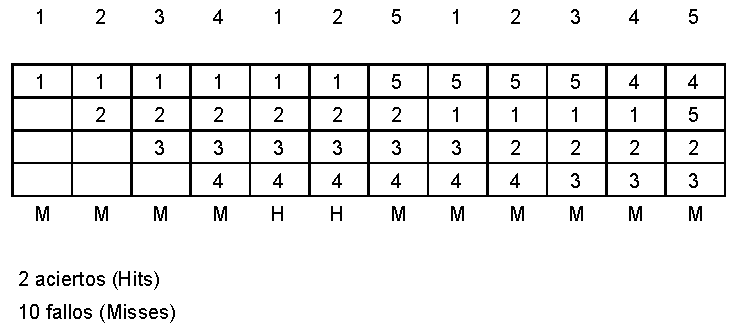
\includegraphics[width=0.5\linewidth]{fifo.pdf}
  \end{center}
\end{figure}

\end{document}
